\documentclass[11pt,oneside]{article}	%use"amsart"insteadof"article"forAMSLaTeXformat
\usepackage{geometry}		%Seegeometry.pdftolearnthelayoutoptions.Therearelots.
\geometry{letterpaper}		%...ora4paperora5paperor...
%\geometry{landscape}		%Activateforforrotatedpagegeometry
%\usepackage[parfill]{parskip}		%Activatetobeginparagraphswithanemptylineratherthananindent
\usepackage{graphicx}				%Usepdf,png,jpg,orepsßwithpdflatex;useepsinDVImode
								%TeXwillautomaticallyconverteps-->pdfinpdflatex		
\usepackage{amssymb}
\usepackage{amsmath}
\usepackage[colorlinks]{hyperref}

%----macros begin---------------------------------------------------------------
\usepackage{color}
\usepackage{amsthm}
\usepackage{amsmath}

\def\conv{\mbox{\textrm{conv}\,}}
\def\aff{\mbox{\textrm{aff}\,}}
\def\E{\mathbb{E}}
\def\R{\mathbb{R}}
\def\Z{\mathbb{Z}}
\def\tex{\TeX}
\def\latex{\LaTeX}
\def\v#1{{\bf #1}}
\def\p#1{{\bf #1}}
\def\T#1{{\bf #1}}

\def\vet#1{{\left(\begin{array}{cccccccccccccccccccc}#1\end{array}\right)}}
\def\mat#1{{\left(\begin{array}{cccccccccccccccccccc}#1\end{array}\right)}}

\def\lin{\mbox{\rm lin}\,}
\def\aff{\mbox{\rm aff}\,}
\def\pos{\mbox{\rm pos}\,}
\def\cone{\mbox{\rm cone}\,}
\def\conv{\mbox{\rm conv}\,}
\newcommand{\homog}[0]{\mbox{\rm homog}\,}
\newcommand{\relint}[0]{\mbox{\rm relint}\,}

%----macros end-----------------------------------------------------------------

\title{Boolean combinations of cellular complexes as chain operations
\footnote{This document is part of the \emph{Linear Algebraic Representation with CoChains} (LAR-CC) framework~\cite{cclar-proj:2013:00}. \today}
}
\author{Alberto Paoluzzi}
%\date{}							%Activatetodisplayagivendateornodate

\begin{document}
\maketitle
\tableofcontents
\nonstopmode

%-------------------------------------------------------------------------------
\section{Introduction}
%-------------------------------------------------------------------------------

In this module a novel approach to Boolean operations of cellular complexes is defined and implemented. The novel algorithm may be summarised as follows. 

First we compute the CDC (Common Delaunay Complex) of the input LAR complexes $A$ and $B$, to get a LAR of the \emph{simplicial} CDC.

Then, we split the cells intersecting the boundary faces of the input complexes, getting the final \emph{polytopal} SCDC  
(Split Common Delaunay Complex), whose cells  provide the  basis for the linear coordinate representation of both input 
complexes, upon the same space decomposition.

Afterwards, every Boolean result is computed by bitwise operations, between the coordinate representations of the transformed $A$ and $B$ input.

Finally a greedy assembly of SCDC cells is executed, in order to return a polytopal complex with a reduced number of cells.



\subsection{Preview of the Boolean algorithm}
%-------------------------------------------------------------------------------

The goal is the computation of $A \diamond B$, with $\diamond\in \{\cup, \cap, -\}$, where a LAR representation of both $A$ and $B$ is given. The Boolean algorithm works as follows.

\begin{enumerate}
\item 
Embed both cellular complexes $A$ and $B$ in the same space (say, identify their common vertices) by $V_{ab} = V_a \cup V_b$.
\item 
Build their CDC  (Common Delaunay Complex) as the LAR of \emph{Delaunay triangulation} of the vertex set $V_{ab}$, and embedded $\partial A$ and $\partial B$ in it.
\item 
Split the (highest-dimensional) cells of CDC crossed by $\partial A$ or $\partial B$. Their lower dimensional faces remain partitioned accordingly. We name the resulting complex SCDC (Split Common Delaunay Complex).
\item 
With respect to the SCDC basis of $d$-cells $C_d$, compute two coordinate chains $\alpha,\beta: C_d \to \{0,1\}$, such that: 
\begin{align}
	\alpha(cell) &= 1  \quad\mbox{if\ } |cell| \subset A;  \quad\mbox{else\ } \alpha(cell) = 0, \nonumber\\
	\beta(cell) &= 1  \quad\mbox{if\ } |cell| \subset B;  \quad\mbox{else\ } \beta(cell) = 0. \nonumber
\end{align}
\item 
Extract accordingly the SCDC chain corresponding to $A \diamond B$, with $\diamond\in \{\cup, \cap, -\}$.
\end{enumerate}


\subsection{Remarks}
%-------------------------------------------------------------------------------

You may  make an analogy between the SCDC (\emph{Split} CDC) and a CDT (Constrained Delaunay Triangulation).  In part they coincide, but in general, the SCDC is a polytopal complex, and is not a simplicial complex as the CDC.

The more complex algorithmic step is the cell splitting.  
Every time, a single $d$-cell  $c$  is split by a single hyperplane (cutting its interior)  giving either two splitted cells $c_1$ and $c_2$, or just one output cell (if the hyperplane is the affine hull of the CDC facet)
whatever the input cell dimension $d$.  After every splitting of the cell interior, the row $c$ is substituted (within the \texttt{CV} matrix) by $c_1$, and $c_2$ is 
added to the end of the \texttt{CV} matrix, as a new row.

The splitting process is started by ``splitting seeds" generated by $(d-1)$-faces of both operand boundaries.
In fact, every such face, say $f$, has vertices on CDC and \emph{may} split some incident CDC $d$-cell.  In particular, starting from its vertices,
$f$ must split the CDC cells in whose interior it passes though.

So, a dynamic data structure is set-up, storing for each boundary face $f$ the list of cells it must cut, and, for every CDC $d$-cell with interior traversed
by some such $f$, the list of cutting faces.  This data structure is continuously updated during the splitting process, using the 
adjacent cells of the split ones, who are to be split in turn.  Every split cell may add some adjacent cell to be split, and after the split,
the used pair (\texttt{cell,face}) is removed.  The splitting process continues until the data structure becomes empty.

Every time a cell is split, it is characterized as either internal (1) or external (0) to the used (oriented) boundary facet f, so that the two 
resulting subcells $c_1$ and $c_2$  receive two opposite characterization (with respect to the considered boundary).

At the very end, every (polytopal) SCDC $d$-cell has two bits of information (one for argument $A$ and one for argument $B$), telling whether it is internal  (1) or external (0) or unknown (-1) with respect to every Boolean argument.

A final recursive traversal of the SCDC, based on cell adjacencies, transforms every $-1$ into either 0 or 1, providing the two final chains to be bitwise operated, depending on the Boolean operation to execute.


%-------------------------------------------------------------------------------
\section{Step 1: merging discrete spaces}
%-------------------------------------------------------------------------------


\subsection{Requirements}
%-------------------------------------------------------------------------------

The \emph{join} of two sets $P, Q \subset \E^d$ is the set $PQ = \{\alpha \v{x} + \beta \v{y}\,| \v{x} \in P,\  \v{y} \in Q\}$,
where $\alpha, \beta \in \R$, $\alpha, \beta \geq 0$, and $\alpha + \beta = 1$. The join operation is associative and commutative.


\paragraph{Input} 
Two LAR models of two non-empty ``solid'' $d$-spaces $A$ and $B$, denoted as \texttt{(V1,CV1)} and \texttt{(V2,CV2)}. 


\paragraph{Output} 
The LAR representation \texttt{(V,CV)} of Delaunay triangulation (simplicial $d$-complex) of the set $\conv AB \subset \E^d$, convex hull of the join of $A$ and $B$, named Common Delaunay Complex (CDC) in the following.

\paragraph{Auxiliary data structures} 
This software module returns also:

\begin{enumerate}
\item 
a dictionary \texttt{vertDict} of \texttt{V} vertices, with \emph{key} the symbolic representation of vertices \texttt{v} returned by expressions \texttt{vcode(v)}, $\texttt{v}\in \texttt{V}$, and with values the finite ordinal numbers of the vertices;

\item 
the numbers \texttt{n1}, \texttt{n12}, \texttt{n2} of the elements of \texttt{V1}, $\texttt{V1}\cap\texttt{V2}$, and \texttt{V2}, respectively. Notice that the following assertions must hold (see Figure~\ref{fig:bounds}):
\begin{align}
\texttt{n1} - \texttt{n12} + \texttt{n2} &= \texttt{n} \\
0 < \texttt{n} - \texttt{n2}  &\leq  \texttt{n1}  <  \texttt{n} 
\end{align}

\item the input boundary complex \texttt{(V,BC)}, with $\texttt{BC} = \texttt{BC1+BC2}$, i.e.~the union of the  two boundary $(d-1)$-complexes \texttt{(V,BC1)} and \texttt{(V,BC2)}, defined on the common vertices.
\end{enumerate}

\begin{figure}[htbp] %  figure placement: here, top, bottom, or page
   \centering
   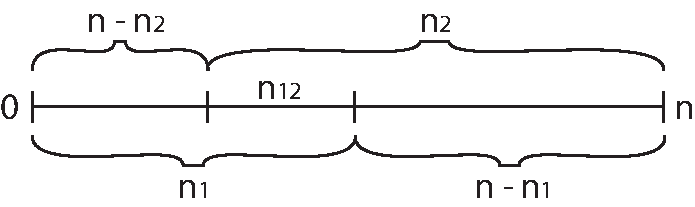
\includegraphics[width=0.5\linewidth]{images/bounds} 
   \caption{Relationships inside the orderings of CDC vertices}
   \label{fig:bounds}
\end{figure}

\subsection{Implementation}
%-------------------------------------------------------------------------------


\subsubsection{Summary}

%-------------------------------------------------------------------------------
@D First Boolean step
@{""" First Boolean step """
def larBool1():
	V, CV1,CV2, n1,n12,n2 = mergeVertices(model1,model2)
	VV = AA(LIST)(range(len(V)))
	V,CV,vertDict,n1,n12,n2,BC,nbc1,nbc2 = makeCDC(arg1,arg2, brep)
	W,CW,VC,BCellCovering,cellCuts,boundary1,boundary2,BCW = makeSCDC(V,CV,BC,nbc1,nbc2)
	assert len(VC) == len(V) 
	assert len(BCellCovering) == len(BC)
	return W,CW,VC,BCellCovering,cellCuts,boundary1,boundary2,BCW 
@}
%-------------------------------------------------------------------------------

\subsubsection{Detail functions}


%-------------------------------------------------------------------------------
@D Compute model boundaries of complex of convex cells
@{""" Compute model boundaries of complex of convex cells """

def larFacetsOfPolytopalComplex(vertDict,cells,facets):
	(V1,CV1),(V2,CV2) = model1,model2
	for cell in CV1:
		Vcell = [V1[v] for v in cell]

@}
%-------------------------------------------------------------------------------


%-------------------------------------------------------------------------------
@D Merge two dictionaries with keys the point locations
@{""" Merge two dictionaries with keys the point locations """
def mergeVertices(model1, model2):

	(V1,CV1),(V2,CV2) = model1, model2

	n = len(V1); m = len(V2)
	def shift(CV, n): 
		return [[v+n for v in cell] for cell in CV]
	CV2 = shift(CV2,n)

	vdict1 = defaultdict(list)
	for k,v in enumerate(V1): vdict1[vcode(v)].append(k) 
	vdict2 = defaultdict(list)
	for k,v in enumerate(V2): vdict2[vcode(v)].append(k+n) 
	vertDict = defaultdict(list)
	for point in vdict1.keys(): vertDict[point] += vdict1[point]
	for point in vdict2.keys(): vertDict[point] += vdict2[point]

	case1, case12, case2 = [],[],[]
	for item in vertDict.items():
		key,val = item
		if len(val)==2:  case12 += [item]
		elif val[0] < n: case1 += [item]
		else: case2 += [item]
	n1 = len(case1); n2 = len(case12); n3 = len(case2)

	invertedindex = list(0 for k in range(n+m))
	for k,item in enumerate(case1):
		invertedindex[item[1][0]] = k
	for k,item in enumerate(case12):
		invertedindex[item[1][0]] = k+n1
		invertedindex[item[1][1]] = k+n1
	for k,item in enumerate(case2):
		invertedindex[item[1][0]] = k+n1+n2

	V = [eval(p[0]) for p in case1] + [eval(p[0]) for p in case12] + [eval(
				p[0]) for p in case2]
	CV1 = [sorted([invertedindex[v] for v in cell]) for cell in CV1]
	CV2 = [sorted([invertedindex[v] for v in cell]) for cell in CV2]

	return V,CV1,CV2, n1+n2,n2,n2+n3
@}
%-------------------------------------------------------------------------------




	
%-------------------------------------------------------------------------------
@D Make Common Delaunay Complex
@{""" Make Common Delaunay Complex """
def makeCDC(arg1,arg2, brep):

	(V1,basis1), (V2,basis2) = arg1,arg2
	(facets1,cells1),(facets2,cells2) = basis1[-2:],basis2[-2:]
	model1, model2 = (V1,cells1),(V2,cells2)

	V, _,_, n1,n12,n2 = mergeVertices(model1, model2)
	n = len(V)
	assert n == n1 - n12 + n2
	
	CV = sorted(AA(sorted)(Delaunay(array(V)).simplices))
	
	vertDict = defaultdict(list)
	for k,v in enumerate(V): vertDict[vcode(v)] += [k]
	
	if brep == False:
    	signs1,BC1 = signedCellularBoundaryCells(V1,basis1)
    	
    	BC1pairs = zip(*signedCellularBoundaryCells(V1,basis1))
    	BC1 = [basis1[-2][face] if sign>0 else swap(basis1[-2][face]) for (sign,face) in BC1pairs]
    
    	BC2pairs = zip(*signedCellularBoundaryCells(V2,basis2))
    	BC2 = [basis2[-2][face] if sign>0 else swap(basis2[-2][face]) for (sign,face) in BC2pairs] 

	else:
		BC1,BC2 = basis1[-1],basis2[-1]
    
	BC = [[ vertDict[vcode(V1[v])][0] for v in cell] for cell in BC1] + [ 
			[ vertDict[vcode(V2[v])][0] for v in cell] for cell in BC2] #+ qhullBoundary(V)
		
	
	return V,CV,vertDict,n1,n12,n2,BC,len(BC1),len(BC2)
@}
%-------------------------------------------------------------------------------




%-------------------------------------------------------------------------------
\section{Step 2: splitting cells}
%-------------------------------------------------------------------------------

The goal of this section is to transform the CDC simplicial complex, into the polytopal Split Common Delaunay Complex (SCDC), by splitting the $d$-cells of CDC crossed in their interior by some cell of the input boundary complex.

\subsection{Requirements}
%-------------------------------------------------------------------------------
We call here for a sequential implementation, following every $(d-1)$-facet \texttt{lambda} in \texttt{BC} (for \emph{Boundary Cells}). We start the splitting with \texttt{COVECTOR(lambda)} from \texttt{cell}, one of the CDC $d$-cells  incident on a vertex of \texttt{lambda}, and continue the splitting on the $d$-cells $(d-1)$-adjacent  to \texttt{cell}, where (a) \texttt{COVECTOR(lambda)} either crosses the \texttt{cell}'s interior or contains one of \texttt{cell}'s $(d-1)$-facets \and{and} (b) such that the intersection with \texttt{lambda} is not empty, until the queue (or stack) of $d$-cells to intersect with \texttt{covector} is not empty.

\paragraph{Best computational strategy}
First associate to each cutting facet the list of cells it may cut; then execute all the cuts. In this way we can compute the adjacency matrix just one time at the beginning of the procedure, and do not need to update it after every split.

\paragraph{Input}
The output of previous algorithm stage.

\paragraph{Output}
The LAR representation \texttt{(W,PW)} of the SCDC,

\paragraph{Auxiliary data structures} 
This software module returns also
 a dictionary \texttt{splitFacets}, with keys the  input boundary faces and values the list of pairs\texttt{(covector,fragmentedFaces)}.   


\subsection{Implementation}
%-------------------------------------------------------------------------------

\subsubsection{Summary}

%-------------------------------------------------------------------------------
@D Second Boolean step
@{""" Second Boolean step """
def larBool2(boundary1,boundary2):
	dim = len(W[0])
	WW = AA(LIST)(range(len(W)))
	FW = larConvexFacets (W,CW)
	_,EW = larFacets((W,FW), dim=2)
	boundary1,boundary2,FWdict = makeFacetDicts(FW,boundary1,boundary2)
	if dim == 3: 
		_,EW = larFacets((W,FW), dim=2)
		bases = [WW,EW,FW,CW]
	elif dim == 2: bases = [WW,FW,CW]
	else: print "\nerror: not implemented\n"
	return W,CW,dim,bases,boundary1,boundary2,FW,BCW
@}
%-------------------------------------------------------------------------------

\subsubsection{Detail functions}


\paragraph{Computing the adjacent cells of a given cell}
To perform this task we make only use of the \texttt{CV} list. In a more efficient implementation we should make direct use of the sparse adjacency matrix, to be dynamically updated together with the \texttt{CV} list.
The computation of the adjacent $d$-cells of a single $d$-cell is given here by extracting a column of the $\texttt{CSR}(M_d\, M_d^t)$. This can be done by multiplying $\texttt{CSR}(M_d)$ by its transposed row corresponding to the query $d$-cell. 

%-------------------------------------------------------------------------------
@D Computing the adjacent cells of a given cell
@{""" Computing the adjacent cells of a given cell """
def adjacencyQuery (V,CV):
	dim = len(V[0])
	csrCV =  csrCreate(CV)
	csrAdj = matrixProduct(csrCV,csrTranspose(csrCV))
	def adjacencyQuery0 (cell):
		nverts = len(CV[cell])
		cellAdjacencies = csrAdj.indices[csrAdj.indptr[cell]:csrAdj.indptr[cell+1]]
		return [acell for acell in cellAdjacencies if dim <= csrAdj[cell,acell] < nverts]
	return adjacencyQuery0
@}
%-------------------------------------------------------------------------------


\paragraph{Relational inversion (characteristic matrix transposition)}

The operation could be executed by simple matrix transposition of the CSR (Compressed Sparse Row) representation of the sparse characteristic matrix $M_d \equiv \texttt{CV}$.
A simple relational inversion using Python lists is given here. The \texttt{invertRelation} function 
is given here, linear in the size of the \texttt{CV} list, where the complexity of each cell is constant and 
small in most cases.

%-------------------------------------------------------------------------------
@D Characteristic matrix transposition
@{""" Characteristic matrix transposition """
def invertRelation(CV):
	def myMax(List):
		if List==[]: return -1
		else: return max(List)
	columnNumber = max(AA(myMax)(CV))+1
	VC = [[] for k in range(columnNumber)]
	for k,cell in enumerate(CV):
		for v in cell:
			VC[v] += [k]
	return VC
@}
%-------------------------------------------------------------------------------


\paragraph{Computation of splitting tests}

In order to compute, in the simplest and more general way, whether each of the two split $d$-cells is internal or external to the splitting boundary $d-1$-facet, it is necessary to consider the oriented covector $\phi$ (or one-form) canonically associated to the facet $f$ by the covector representation theorem, i.e.~the corresponding oriented hyperplane. In this case, the internal/external attribute of the split cell will be computed by evaluating the pairing $<v,\phi>$.

%-------------------------------------------------------------------------------
@D Splitting tests
@{""" Splitting tests """
def testingSubspace(V,covector):
	def testingSubspace0(vcell):
		inout = SIGN(sum([INNERPROD([[1.]+V[v],covector]) for v in vcell]))
		return inout
	return testingSubspace0
	
def cuttingTest(covector,polytope,V):
	signs = [INNERPROD([covector, [1.]+V[v]]) for v in polytope]
	signs = eval(vcode(signs))
	return any([value<-0.001 for value in signs]) and \
			any([value>0.001 for value in signs])
	
def tangentTest(covector,facet,adjCell,V):
	common = list(set(facet).intersection(adjCell))
	signs = [INNERPROD([covector, [1.]+V[v]]) for v in common]
	count = 0
	for value in signs:
		if -0.0001<value<0.0001: count +=1
	if count >= len(V[0]): 
		return True
	else: 
		return False	
@}
%-------------------------------------------------------------------------------




\paragraph{Elementary splitting test}

Let us remember that the adjacency matrix between $d$-cells is computed via SpMSpM multiplication by the double application 
\[
\texttt{adjacencyQuery(V,CV)(cell)}, 
\] 
where the first application \texttt{adjacencyQuery(V,CV)}
returns a partial function with bufferisation of the adjacency matrix, and the second application to \texttt{cell} returns the list of adjacent $d$-cells sharing with it a $(d-1)$-dimensional facet.

%-------------------------------------------------------------------------------
@D Elementary splitting test
@{
@< Splitting tests @>

""" Elementary splitting test """
def dividenda(V,CV, cell,facet,covector,unchosen):
	out = []
	adjCells = adjacencyQuery(V,CV)(cell)
	for adjCell in set(adjCells).difference(unchosen):
		if (cuttingTest(covector,CV[adjCell],V) and \
			cellFacetIntersecting(facet,adjCell,covector,V,CV)) or \
			tangentTest(covector,facet,CV[adjCell],V): out += [adjCell]
	return out
@}
%-------------------------------------------------------------------------------

\paragraph{CDC cell splitting with one or more facets}

When splitting a $d$-cell with some hyperplanes, we need to return not only either the two cut parts or the cell itself when the hyperplane is tangent to a $(d-1)$-face, but also the facet lying on the hyperplane. 
In the first cade it is directly computed by the \texttt{SPLITCELL} function, and returned as the \texttt{equal} set of points. In the second case, the cell is transformed by the map that sends the hyperplane in the $x_d=0$ subspace ($z=0$ in 3D), and the searched facet is returned as the (back-transformed) set of cell vertices on this subspace. 

Actually, the process is strongly complicated by the fact that the input cell (and its facets) may be cut by several hyperplanes. By now, we resort to the simplex computation, even if more time-expensive:  to compare each vertex of each cell fragment, against every hyperplanes. This approach will adapt well to the writing of a computational kernel on the GPU.

%-------------------------------------------------------------------------------
@D CDC cell splitting with one or more cutting facets
@{""" CDC cell splitting with one or more cutting facets """
def fragment(cell,cellCuts,V,CV,BC):
	vcell = CV[cell]
	cellFragments = [[V[v] for v in vcell]]
	
	for f in cellCuts[cell]:
		facet = BC[f]
		plane = COVECTOR([V[v] for v in facet])
		for k,fragment in enumerate(cellFragments):
		
			#if not tangentTest(plane,facet,fragment,V):
			[below,equal,above] = SPLITCELL(plane,fragment,tolerance=1e-4,ntry=4)
			if below != above:
				cellFragments[k] = below
				cellFragments += [above]
		facets = facetsOnCuts(cellFragments,cellCuts,V,BC)
	return cellFragments
@}
%-------------------------------------------------------------------------------

\paragraph{SCDC splitting with every boundary facet}
The function \texttt{makeSCDC} is used  to compute the LAR model \texttt{(W,CW)} of the SCDC.
It takes as input the LAR model \texttt{(V,CV)} of the CDC, and the LAR model \texttt{(V,BC)} of the input Boolean Complex, and returns both a new LAR model \texttt{(W,CW)} and the vertex-cell relation \texttt{VC}, i.e.~the transposed of \texttt{CV}.

For every $\texttt{k} \in \texttt{BC}$, a list \texttt{cellsToSplit}

%-------------------------------------------------------------------------------
@D SCDC splitting with every boundary facet
@{""" SCDC splitting with every boundary facet """
def makeSCDC(V,CV,BC,nbc1,nbc2):
	index,defaultValue = -1,-1
	VC = invertRelation(CV)
	CW,BCfrags = [],[]
	Wdict = dict()
	BCellcovering = boundaryCover(V,CV,BC,VC)

	cellCuts = invertRelation(BCellcovering)
	for k in range(len(CV) - len(cellCuts)): cellCuts += [[]]
	
	def verySmall(number): return abs(number) < 10**-5.5
	
	for k,frags in enumerate(cellCuts):
		if cellCuts[k] == []:
			cell = []
			for v in CV[k]:
				key = vcode(V[v])
				if Wdict.get(key,defaultValue) == defaultValue:
					index += 1
					Wdict[key] = index
					cell += [index]
				else: 
					cell += [Wdict[key]]
			CW += [cell]
		else:
			cellFragments = fragment(k,cellCuts,V,CV,BC)
			for cellFragment in cellFragments:
				cellFrag = []
				for v in cellFragment:
					key = vcode(v)
					if Wdict.get(key,defaultValue) == defaultValue:
						index += 1
						Wdict[key] = index
						cellFrag += [index]
					else: 
						cellFrag += [Wdict[key]]
				CW += [cellFrag]	
				
				BCfrags += [ (h, [Wdict[vcode(w)] for w in cellFragment if verySmall( 
								PROD([ COVECTOR( [V[v] for v in BC[h]] ), [1.]+w ])) ] )
							 for h in cellCuts[k]]	
	
	BCW = [ [ Wdict[vcode(V[v])] for v in cell ] for cell in BC]
	W = sorted(zip( Wdict.values(), Wdict.keys() ))
	W = AA(eval)(TRANS(W)[1])
	dim = len(W[0])
	boundary1,boundary2 = boundaryEmbedding(BCfrags,nbc1,dim)
	return W,CW,VC,BCellcovering,cellCuts,boundary1,boundary2,BCW
@}
%-------------------------------------------------------------------------------

%-------------------------------------------------------------------------------
@D Boolean argument boundaries embedding in SCDC
@{""" Boolean argument boundaries embedding in SCDC """
def boundaryEmbedding(BCfrags,nbc1,dim):
	boundary1,boundary2 = defaultdict(list),defaultdict(list)						 
	for h,frags in BCfrags:
		if h < nbc1: boundary1[h] += [frags]
		else: boundary2[h] += [frags]	
	boundarylist1,boundarylist2 = [],[]
	for h,facets in boundary1.items():
		boundarylist1 += [(h, AA(eval)(set([str(sorted(f)) 
							for f in facets if len(set(f)) >= dim])) )]
	for h,facets in boundary2.items():
		boundarylist2 += [(h, AA(eval)(set([str(sorted(f)) 
							for f in facets if len(set(f)) >= dim])) )]
	boundary1,boundary2 = dict(boundarylist1),dict(boundarylist2)
	return boundary1,boundary2
@}
%-------------------------------------------------------------------------------


%-------------------------------------------------------------------------------
@D Make facets dictionaries
@{""" Make facets dictionaries """
def makeFacetDicts(FW,boundary1,boundary2):
	FWdict = dict()
	for k,facet in enumerate (FW): FWdict[str(facet)] = k
	for key,value in boundary1.items():
		value = [FWdict[str(facet)] for facet in value]
		boundary1[key] = value
	for key,value in boundary2.items():
		value = [FWdict[str(facet)] for facet in value]
		boundary2[key] = value
	return boundary1,boundary2,FWdict
@}
%-------------------------------------------------------------------------------


\paragraph{Computation of boundary facets covering with CDC cells}

%-------------------------------------------------------------------------------
@D Computation of boundary facets covering with CDC cells
@{""" Computation of boundary facets covering with CDC cells """
def boundaryCover(V,CV,BC,VC):
	cellsToSplit = list()
	boundaryCellCovering = []
	for k,facet in enumerate(BC):
		covector = COVECTOR([V[v] for v in facet])
		seedsOnFacet = VC[facet[0]]
		cellsToSplit = [dividenda(V,CV, cell,facet,covector,[]) 
							for cell in seedsOnFacet ]
		cellsToSplit = set(CAT(cellsToSplit))
		while True:
			newCells = [dividenda(V,CV, cell,facet,covector,cellsToSplit) 
							for cell in cellsToSplit ]
			if newCells != []: newCells = CAT(newCells)
			covering = cellsToSplit.union(newCells)
			if covering == cellsToSplit: 
				break
			cellsToSplit = covering
		boundaryCellCovering += [list(covering)]
	return boundaryCellCovering
@}
%-------------------------------------------------------------------------------

\paragraph{Cell-facet intersection test}

%-------------------------------------------------------------------------------
@D Cell-facet intersection test
@{""" Cell-facet intersection test """
def cellFacetIntersecting(boundaryFacet,cell,covector,V,CV):
	points = [V[v] for v in CV[cell]]
	vcell1,newFacet,vcell2 = SPLITCELL(covector,points,tolerance=1e-4,ntry=4)
	boundaryFacet = [V[v] for v in boundaryFacet]
	translVector = boundaryFacet[0]
	
	# translation 
	newFacet = [ VECTDIFF([v,translVector]) for v in newFacet ]
	boundaryFacet = [ VECTDIFF([v,translVector]) for v in boundaryFacet ]
	
	# linear transformation: boundaryFacet -> standard (d-1)-simplex
	d = len(V[0])
	transformMat = mat( boundaryFacet[1:d] + [covector[1:]] ).T.I
	
	# transformation in the subspace x_d = 0
	newFacet = (transformMat * (mat(newFacet).T)).T.tolist()
	boundaryFacet = (transformMat * (mat(boundaryFacet).T)).T.tolist()
	
	# projection in E^{d-1} space and Boolean test
	newFacet = MKPOL([ AA(lambda v: v[:-1])(newFacet), 
							[range(1,len(newFacet)+1)], None ])
	boundaryFacet = MKPOL([ AA(lambda v: v[:-1])(boundaryFacet), 
							[range(1,len(boundaryFacet)+1)], None ])
	verts,cells,pols = UKPOL(INTERSECTION([newFacet,boundaryFacet]))
	
	if verts == []: return False
	else: return True
@}
%-------------------------------------------------------------------------------








%-------------------------------------------------------------------------------
\section{Step 3: cell labeling}
%-------------------------------------------------------------------------------

The goal of this stage is to label every cell of the SCDC with two bits, corresponding to the input spaces $A$ and $B$, and telling whether the cell is either internal (1) or external (0) to either spaces.

\subsection{Requirements}
%-------------------------------------------------------------------------------


\paragraph{Input}
The output of previous algorithm stage.

\paragraph{Output}
The array \texttt{cellLabels} with \emph{shape} $\texttt{len(PW)}\times 2$, and values in $\{0,1\}$.


\subsection{Implementation}
%-------------------------------------------------------------------------------

The labelling of LAR of the SCDC may be decomposed in five consecutive steps. The first step was actually executed during the splitting stage, by accumulating a single facet of every split cells embedded on the affine hull (the covector hyperplane) of the splitting boundary \texttt{facet}. The second  step provides the computation of the sparse matrix of the linear coboundary operator $\delta_{d-1}: C_{d-1} \to C_d$.
The third step operates upon the previous two pieces of information, in order to compute the coboundary chain of the boundary chain of both input Boolean arguments.
The fourth step attaches a \textsc{in/out} label to each $d$-cell of the previously computed $d$-chain.
Finally, the fifth step spreads around the labels to cover all the $d$-cells of SCDC. This knowledge allows for the computation of every interesting Boolean expressions between the input complexes.

\subsubsection{Summary}

%-------------------------------------------------------------------------------
@D Third Boolean step
@{""" Third Boolean step """
def larBool3():
	coBoundaryMat = signedCellularBoundary(W,bases).T
	boundaryMat = coBoundaryMat.T
	CWbits = [[-1,-1] for k in range(len(CW))]
	CWbits = cellTagging(boundary1,boundaryMat,CW,FW,W,BCW,CWbits,0)
	CWbits = cellTagging(boundary2,boundaryMat,CW,FW,W,BCW,CWbits,1)
	for cell in range(len(CW)):
		if CWbits[cell][0] == 1:
			CWbits = booleanChainTraverse(0,cell,W,CW,CWbits,1)		
		if CWbits[cell][0] == 0:
			CWbits = booleanChainTraverse(0,cell,W,CW,CWbits,0)
		if CWbits[cell][1] == 1:
			CWbits = booleanChainTraverse(1,cell,W,CW,CWbits,1)
		if CWbits[cell][1] == 0:
			CWbits = booleanChainTraverse(1,cell,W,CW,CWbits,0)
	chain1,chain2 = TRANS(CWbits)
	return W,CW,FW,boundaryMat,boundary1,boundary2,chain1,chain2,CWbits
@}
%-------------------------------------------------------------------------------

\subsubsection{Detail functions}



\paragraph{Computation of boundary cells embedded in SCDC}

%-------------------------------------------------------------------------------
@D Computation of embedded boundary cells
@{""" Computation of embedded boundary cells """
def facetsOnCuts(cellFragments,cellCuts,V,BC):


	pass
	return #facets
@}
%-------------------------------------------------------------------------------


\paragraph{Coboundary operator on SCDC space decomposition}

In this section we develop a stronger characterisation of the boundaries, by fully tagging in SCDC the internal coboundary of boundaries of $A$ and $B$ Boolean arguments. This novel strategy should allow the recursive tagging extension to work correctly in all cases.

As we know, the  coboundary operators $\delta_{k-1}: C_{k-1} \to C_k$ are the transpose of the boundary operators $\partial_k: C_k \to C_{k-1}$ ($1\leq k\leq d$). We therefore proceed to the construction of the operator $\delta_{d-1}$, according to the procedure illustrated in~\cite{}. For this purpose we need to use both the $C_d$ and the $C_{d-1}$ bases of SCDC. The first basis is generated as \texttt{CV} array during the splitting. The second basis will be built from $C_d$ using the proper $d$-adjacency algorithm from~\cite{}. 

Let us remember that a (co)boundary operator may be applied to \emph{any} chain from the linear space of chains defined upon a cellular complex. 
In our case we have already generated the $(d-1)$-chains $\partial A$ and $\partial B$ while building the SCDC, by accumulating, in the course of the splitting phase, the $(d-1)$-facets discovered while tracking the boundaries of $A$ and $B$. We just need now to tag (a subset of) $\delta_{d-1}\partial_d A$ and $\delta_{d-1}\partial_d B$.

%-------------------------------------------------------------------------------
@D Coboundary operator on the convex decomposition of common space
@{""" Coboundary operator on the convex decomposition of common space """
from scipy.spatial import ConvexHull
def qhullBoundary(V):
	points = array(V)
	hull = ConvexHull(points)
	out = hull.simplices.tolist()
	return sorted(out)

""" Extracting a $(d-1)$-basis of SCDC """
"""
def convexBoundary(V):
	covectors = defaultdict(list)
	tri = Delaunay(V)
	FV = tri.convex_hull.tolist()
	

def larConvexFacets (V,CV):
	dim = len(V[0])
	model = V,CV
	V,FV = larFacets(model,dim)
	FV = AA(eval)(list(set(AA(str)(FV + convexBoundary(V,CV)))))
	FV = sorted(AA(sorted)(FV))
	return FV
"""
def larConvexFacets(Y,CY):
	FY = set()
	for cell in CY:
		cellVerts = array([[Y[v],v] for v in cell])	   # v globale
		cellVerts,cellVertsInd = TRANS(cellVerts)
		covectors = defaultdict(list) 
		tri = Delaunay(cellVerts)   # struttura dati
		FV = tri.convex_hull.tolist()   # facce con indici vertici LOCALI
		for k,facet in enumerate(FV):
			covect = list(COVECTOR([cellVerts[v] for v in facet]))
			normalizedCovect = [ h*SIGN(covect[0])  for h in covect]
			for h,comp in enumerate(UNITVECT(normalizedCovect)): 
				if not isclose(0.0, comp): 
					theSign = SIGN(comp)
					break
			normalizedCovect = [x*theSign  if x!=abs(0.0) else x for x in normalizedCovect]
			covectors[vcode(normalizedCovect)] += [k]
		for covector,facets in covectors.items():
			localFacets = [list(set(CAT([FV[facet] for facet in facets])))]
			for facet in localFacets:
				FY = FY.union([tuple([ cellVertsInd[v] for v in facet ])])	
	#for facet in convexBoundary(Y,CY):			
	#	FY = FY.union(facet)	
	FY = sorted(list(AA(sorted)(AA(list)(FY))))
	return FY	

if __name__ == "__main__":
    V,CV = larCuboids((2,2,2))
    FV = larConvexFacets(V,CV)
    # EV = larConvexFacets(V,FV)
    submodel = SKEL_1(STRUCT(MKPOLS((V,FV))))
    VV = AA(LIST)(range(len(V)))
    VIEW(larModelNumbering(1,1,1)(V,[VV,FV,CV],submodel,1.5))
@}
%-------------------------------------------------------------------------------


\paragraph{Computation of boundary operator}

The computation of the boundary operator $\partial_d$ on the SCDC $d$-basis \texttt{(W,CW)} requires the knowledge of the $(d-1)$-basis \texttt{(W,FW)}. The goal of this section is hence the---partially incremental---computation of \texttt{FW}. This set can be partitioned into \emph{internal} cells, that have 2 cofaces, and \emph{boundary} cells, that have only 1 coface. The first subset is easily computed by the \texttt{larFacets} function; the computation of the second subset requires some more work, specified in the following.

First, we compute the 0-chain of boundary vertices of the SCDC, using \emph{qHull}, and take advantage of the \texttt{CV} matrix to extract the chain of $d$-cells sharing with the boundary a $(d-1)$facet. Second, using the \emph{partial} boundary operator generated by using only the interior $(d-1)$-facets, and the associated $(d-2)$-boundary operator, we select the sub-chain made by the non-closed $d$-cells of this subset. Third, the boundary facet of each of them is finally selected, added to the $(d-1)$-basis of SCDC, and the corresponding row is added at the bottom line of the matrix of $\partial_{d-1}$.

%-------------------------------------------------------------------------------
@D Computation of boundary operator of a convex LAR model
@{""" Computation of boundary operator of a convex LAR model"""
def convexBoundary(W,CW):
	points = array(W)
	hull = ConvexHull(points,qhull_options="Qc")
	coplanarVerts = hull.coplanar.tolist()
	if coplanarVerts != []:  coplanarVerts = CAT(coplanarVerts)
	BWchain = set( CAT(qhullBoundary(W)) + coplanarVerts )
	dim = len(W[0])
	bfacets = [list(BWchain.intersection(cell)) 
					for cell in CW if len(BWchain.intersection(cell)) >= dim]
	return bfacets
@}
%-------------------------------------------------------------------------------


\paragraph{Coboundary of boundary chains}

%-------------------------------------------------------------------------------
@D Coboundary of boundary chain
@{""" Coboundary of boundary chain """
@}
%-------------------------------------------------------------------------------


\paragraph{Labeling seeds}

%-------------------------------------------------------------------------------
@D Writing labelling seeds on SCDC
@{""" Writing labelling seeds on SCDC """
def cellTagging(boundaryDict,boundaryMat,CW,FW,W,BC,CWbits,arg):
	dim = len(W[0])
	for face in boundaryDict:
		for facet in boundaryDict[face]:
			cofaces = list(boundaryMat[facet].tocoo().col)
			if len(cofaces) == 1: 
				CWbits[cofaces[0]][arg] = 1
			elif len(cofaces) == 2:
				v0 = list(set(CW[cofaces[0]]).difference(FW[facet]))[0]
				v1 = list(set(CW[cofaces[1]]).difference(FW[facet]))[0]
				# take d affinely independent vertices in face (TODO: use pivotSimplices() 
				simplex0 = BC[face][:dim] + [v0]
				simplex1 = BC[face][:dim] + [v1]
				sign0 = sign(det([W[v]+[1] for v in simplex0]))
				sign1 = sign(det([W[v]+[1] for v in simplex1]))
				
				if sign0 == 1: CWbits[cofaces[0]][arg] = 1
				elif sign0 == -1: CWbits[cofaces[0]][arg] = 0
				if sign1 == 1: CWbits[cofaces[1]][arg] = 1
				elif sign1 == -1: CWbits[cofaces[1]][arg] = 0
			else: 
				print "error: too many cofaces of boundary facets"
	return CWbits
@}
%-------------------------------------------------------------------------------


\paragraph{Recursive diffusion of labels}
A recursive function \texttt{booleanChainTraverse} is given in the script below, where 

%-------------------------------------------------------------------------------
@D Recursive diffusion of labels on SCDC
@{""" Recursive diffusion of labels on SCDC """
def booleanChainTraverse(h,cell,V,CV,CWbits,value):
	adjCells = adjacencyQuery(V,CV)(cell)
	for adjCell in adjCells: 
		if CWbits[adjCell][h] == -1:
			CWbits[adjCell][h] = value
			CWbits = booleanChainTraverse(h,adjCell,V,CV,CWbits,value)
	return CWbits
@}
%-------------------------------------------------------------------------------



%-------------------------------------------------------------------------------
\section{Step 4: greedy cell gathering}
%-------------------------------------------------------------------------------

The goal of this stage is to make as lower as possible the number of cells in the  output LAR of the space $AB$, partitioned into convex cells.

\paragraph{Input}
The LAR model \texttt{(W,PW)} of the SCDC and the array \texttt{cellLabels}.

\paragraph{Output}
The LAR representation \texttt{(W,RW)} of the final fragmented and labeled space $AB$.


\subsection{Requirements}
%-------------------------------------------------------------------------------

The algorithm proposed here for $d$-cell gathering into bigger polytopes is local and greedy. Starting from an initial random $d$-cell, a $(d-1)$-connected $d$-chain is built, by attaching, one at a time, single cells to the boundary of the chain, after (local) verification that the support of the new chain will remain a convex set. 

In case of failure of the test, the facets of the current chain boundary are checked for the gluing of their adjacent and external $d$-coface, until either a new convex is built, or no single cell can be attached convexly, so that the attachment process relative to that chain stops, and its boundary vertices are written in the LAR of a new complex, to gather a single new polytope generated by them. 

Actually, during the stage of boundary checking for finding a new cocell to glue, only a subchain is checked, obtained by subtraction from the boundary of the cutting facets, where attachments are not possible, without
violating the topology of Boolean results. 

Two main algorithm components are needed here. The first one concerns the extraction of the current $d$-chain boundary, the subtraction from it of the splitting facets, and the selection of the facet where to glue another $d$-cell; the second one deals with the convexity test of the candidate (chain $+$ boundary cocell) pair.

The local convexity test will extract, using the (co)boundary matrix of the current chain, the coboundary of the boundary of the candidate facet, and, selected the matrix of hyperplanes associated to it, will compute the centroid of the facet and the vector of signs exposed by the point transformed by right product with this matrix. The local test of convexity is satisfied if and only if all new vertices expose the same signs (or zero), when transformed by this matrix. In other words, the test is satisfied  if all new vertices remain internal (or non external) to the cone generated by such set of boundary hyperplanes.

Every time that a new cell has been selected to join the current chain, the cell is also signed as already used, and hence as no more available for other choices. Of course, the algorithm terminates when all the input  $d$-cells have been selected and signed.


\subsection{Implementation}
%-------------------------------------------------------------------------------
A synthetic view of the simplification process is given by the script below.
The first tool provides a mapping from $(d-1)$-facets of SCDC to their embedding hyperplanes, i.e. to their affine hulls of codimension 1. The second one compute the boundary $(d-1)$-complex of the SCDC $d$-chain currently transformed into a single convex cell. The algorithmic bulk of the simplification process is contained in the script entitled \texttt{Sticking cells together}. The last script provides the high-level interface to transform the generated SCDC into a strongly simplified polytopal complex.

\paragraph{High-level description}

%-------------------------------------------------------------------------------
@D Simplification of the output polytopal complex
@{@< Mapping from facets to hyperplanes @>
@< Building the boundary complex of the current chain @>
@< Sticking cells together @>
@< Gathering and writing a polytopal complex @>
@}
%-------------------------------------------------------------------------------

\subsubsection{Summary}


%-------------------------------------------------------------------------------
@D Fourth Boolean step
@{""" Fourth Boolean step """
def larBool4(W,CWbits):
	W,CX,CXbits = gatherPolytopes(W,CW,FW,boundaryMat,boundary1,boundary2,CWbits)
	FX = larConvexFacets (W,CX)		
	return W,CX,FX,CXbits
@}
%-------------------------------------------------------------------------------

%submodel = SKEL_1(STRUCT(MKPOLS((W,CX))))
%WW = AA(LIST)(range(len(W)))
%VIEW(STRUCT([ submodel, larModelNumbering(1,1,1)(W,[WW,[],CX],submodel,3) ]))
%VIEW(EXPLODE(1.2,1.2,1)([ submodel, larModelNumbering(1.2,1.2,1)(W,[WW,FX],submodel,3) ]))


\subsubsection{Detail functions}




\paragraph{Mapping from facets to hyperplanes}
The function \texttt{facet2covectors} return the list of hyperplane covectors, with first term homogeneous, i.e.~the row vector $(c,a,b)$ for the line equation $ax+by+c=0$, or the row vector $(d,a,b,c)$ for the plane equation $ax+by+cz+d=0$.
%-------------------------------------------------------------------------------
@D Mapping from facets to hyperplanes
@{""" Mapping from hyperplanes to lists of facets """
def facet2covectors(W,FW):
	return [COVECTOR([W[v] for v in facet]) for facet in FW]

def boundaries(boundary1,boundary2):
	return set(CAT(boundary1.values() + boundary2.values()))
@}
%-------------------------------------------------------------------------------

\paragraph{Building the complex of the current chain}
The function \texttt{chain2complex} returns the boundary complex of the current \texttt{chain}, minus the facet in \texttt{constraints}, where non $d$-cell may be attached to the current \texttt{chain}.
It is computed via multiplication between the matrix of boundary operator and the coordinate representation \texttt{chainCoords} of \texttt{chain}. The \texttt{constraint} set is finally subtracted to the result.  

%-------------------------------------------------------------------------------
@D Building the boundary complex of the current chain
@{from scipy.sparse import csc_matrix
""" Building the boundary complex of the current chain """
def chain2complex(W,CW,chain,boundaryMat,constraints):
	chainCoords = csc_matrix((len(CW), 1))
	for cell in chain: chainCoords[cell] = 1
	boundaryCells = set((boundaryMat * chainCoords).tocoo().row)
	envelope = boundaryCells.difference(constraints)
	return envelope,boundaryCells
@}
%-------------------------------------------------------------------------------

\paragraph{Sticking cells together}
%-------------------------------------------------------------------------------
@D Sticking cells together
@{""" Sticking cells together """
@< Testing the convexity of a single added vertex @>
@< Testing the convexity when attaching a cell to a chain @>
@< Elongate a chain while supports a convex set @>
@}
%-------------------------------------------------------------------------------

\paragraph{Testing the convexity of a single added vertex}
A single cell is possibly attached to the boundary envelope of the current \texttt{chain}. In case of success
the function \texttt{protrudeChain} returns \texttt{True}; otherwise returns \texttt{False}. 
%-------------------------------------------------------------------------------
@D Testing the convexity of a single added vertex
@{""" Testing the convexity of a single added vertex """
def pairing(v,w):
	value = PROD([v,w])
	if -0.01 < value < 0.01: return 0
	else: return SIGN(value)

def convexTest(theSigns,vertex,theCone):
	signs = [ pairing( [1]+vertex,covector ) for covector in theCone]
	return all([theSign*sign >= 0 for (theSign,sign) in zip(theSigns,signs)])
@}
%-------------------------------------------------------------------------------

\paragraph{Testing the convexity of current chain}
%-------------------------------------------------------------------------------
@D Testing the convexity when attaching a cell to a chain
@{""" Testing the convexity when attaching a cell to a chain """
def testAttachment(cell,usedCells,theFacet,chain,
					W,CW,FW,boundaryMat,boundaryCells,covectors):
	theFacetVerts = set(FW[theFacet])
	flag = False
	facetRing = [facet for facet in boundaryCells if facet!=theFacet and \
				 len(theFacetVerts.intersection(FW[facet])) >= len(W[0])-1]
	theCone = [covectors[f] for f in facetRing]
	theFacetPivot = CCOMB([W[v] for v in FW[theFacet]])
	theSigns = [ pairing( [1]+theFacetPivot, covector ) for covector in theCone ]
	if not any([sign==0 for sign in theSigns]):
		testingSet = set(CW[cell]).difference(theFacetVerts)
		flag = all([ convexTest(theSigns,W[vertex],theCone) for vertex in testingSet])
	return flag
@}
%-------------------------------------------------------------------------------

\paragraph{Chain elongation while is convex}

%-------------------------------------------------------------------------------
@D Elongate a chain while supports a convex set
@{""" Elongate a chain while supports a convex set """
def protrudeChain (W,CW,FW,chain,boundaryMat,covectors,usedCells,constraints):
	verts = []
	while True:	
		changed = False
		envelope,boundaryCells = chain2complex(W,CW,chain,boundaryMat,constraints)
		for facet in envelope:
			success = False
			chainCoords = csr_matrix((1,len(FW)))
			chainCoords[0,facet] = 1
			cocells = list((chainCoords * boundaryMat).tocoo().col)
			
			if len(cocells)==2:
				if cocells[0] in chain: cell = cocells[1]
				elif cocells[1] in chain: cell = cocells[0]
				if not usedCells[cell]:
					success = testAttachment(cell,usedCells,facet,chain, \
								W,CW,FW,boundaryMat,boundaryCells,covectors)
				if success: 
					changed = True
					usedCells[cell] = True
					chain += [cell]
		if not changed: break		
			
	chainCoords = csc_matrix((len(CW),1))
	for cell in chain: 
		chainCoords[cell,0] = 1
		usedCells[cell] = True
	boundaryFacets = list((boundaryMat*chainCoords).tocoo().row)
	verts = [FW[facet] for facet in boundaryFacets]
	verts = sorted(list(set(CAT(verts))))
	return verts,usedCells
@}
%-------------------------------------------------------------------------------

\paragraph{Gathering and writing a polytopal complex}
The task of the \texttt{gatherPolytopes} function, given below, is to return the LAR \texttt{(X,CX)} of the SCDC \texttt{(W,CW)} generated by the previous phases of the Boolean algorithm, after reducing its representation to a much smaller size, (a) by gathering subsets of cells into single bigger polytopal cells within the characteristic matrix \texttt{CX}, and (b) by assembling their boundary vertices into the (reduced) vertex set \texttt{X}. Of course, while reducing the number of polytopal cells, the procedure should not change the Boolean structure of the input complex, i.e. the support spaces $|C_A|, |C_B|$ of proper chains $C_A$ and $C_B$ and of their Boolean combinations.

%-------------------------------------------------------------------------------
@D Gathering and writing a polytopal complex
@{""" Gathering and writing a polytopal complex """
def gatherPolytopes(W,CW,FW,boundaryMat,bounds1,bounds2,CWbits):
	usedCells = [False for cell in CW]
	covectors = facet2covectors(W,FW)
	constraints = boundaries(bounds1,bounds2)
	Xdict,index,CX,defaultValue,CXbits = dict(),0,[],-1,[]
	while not all(usedCells):
		for k,cell in enumerate(CW):
			if not usedCells[k]:
				chain = [k]
				usedCells[k] = True
				verts,usedCells = protrudeChain(W,CW,FW,chain,boundaryMat,
									covectors,usedCells,constraints)
				CX += [ verts ]
				CXbits += [ CWbits[k] ]
	return W,CX,CXbits
@}
%-------------------------------------------------------------------------------


%-------------------------------------------------------------------------------
\section{The main Boolean procedure}
%-------------------------------------------------------------------------------

\subsection{Goal: generating the Boolean complex}


\subsection{Implementation}


%-------------------------------------------------------------------------------
@D Boolean Algorithm
@{""" Boolean Algorithm """
def larBool(arg1,arg2, brep=False):
	V1,basis1 = arg1
	V2,basis2 = arg2
	cells1 = basis1[-1]
	cells2 = basis2[-1]
	model1,model2 = (V1,cells1),(V2,cells2)
	
	@< First Boolean step @>
	@< Second Boolean step @>
	@< Third Boolean step @>
	@< Fourth Boolean step @>
		
	W,CW,VC,BCellCovering,cellCuts,boundary1,boundary2,BCW = larBool1()
	W,CW,dim,bases,boundary1,boundary2,FW,BCW = larBool2(boundary1,boundary2)
	W,CW,FW,boundaryMat,boundary1,boundary2,chain1,chain2,CWbits = larBool3()
	W,CX,FX,CXbits = larBool4(W,CWbits)
	chain1,chain2 = TRANS(CXbits)
	
	print "\n>>>> W =",W
	print "\n>>>> CX =",CX
	print "\n>>>> FX =",FX
	boundaryMat = boundary(CX,FX)

	def theBoundary(boundaryMat,CX,coords):
		print "\n>>>> boundaryMat =",boundaryMat
		print "\n>>>> coords =",coords
		chainCoords = csc_matrix((len(CX), 1))
		for cell in coords: chainCoords[cell,0] = 1
		boundaryCells = list((boundaryMat * chainCoords).tocoo().row)
		orientations = list((boundaryMat * chainCoords).tocoo().data)
		orientedBoundary = [ FX[face] for (sign,face) in zip(orientations,boundaryCells)  if sign == 1 ]
		return orientedBoundary


	def larBool0(op):	
		if op == "union": 
			ucoords,uchain = TRANS([(k,cell) for k,(cell,c1,c2) in enumerate(zip(CX,chain1,chain2)) if c1+c2>=1])
			return W,CW,uchain,CX,FX,theBoundary(boundaryMat,CX,ucoords)
		elif op == "intersection": 
			icoords,ichain = TRANS([(k,cell) for k,(cell,c1,c2) in enumerate(zip(CX,chain1,chain2)) if c1*c2==1])
			return W,CW,ichain,CX,FX,theBoundary(boundaryMat,CX,icoords)
		elif op == "xor": 
			xcoords,xchain = TRANS([(k,cell) for k,(cell,c1,c2) in enumerate(zip(CX,chain1,chain2)) if c1+c2==1])
			return W,CW,xchain,CX,FX,theBoundary(boundaryMat,CX,xcoords)
		elif op == "difference": 
			dcoords,dchain = TRANS([(k,cell) for k,(cell,c1,c2) in enumerate(zip(CX,chain1,chain2)) if c1==1 and c2==0 ])
			return W,CW,dchain,CX,FX,theBoundary(boundaryMat,CX,dcoords)
		else: print "Error: non implemented op"

	return larBool0
@}
%-------------------------------------------------------------------------------


%-------------------------------------------------------------------------------
\section{LAR simplification}
%-------------------------------------------------------------------------------

Occasionally, we may need to simplify 

%-------------------------------------------------------------------------------
\section{Exporting the library}
%-------------------------------------------------------------------------------


%-------------------------------------------------------------------------------
@O lib/py/bool1.py
@{""" Module for Boolean ops with LAR """
@< Initial import of modules @>
from splitcell import *
DEBUG = False
@< Symbolic utility to represent points as strings @>
@< Merge two dictionaries with keys the point locations @>
@< Make Common Delaunay Complex @>
@< Cell-facet intersection test @>
@< Elementary splitting test @>
@< Computing the adjacent cells of a given cell @>
@< Computation of boundary facets covering with CDC cells @>
@< CDC cell splitting with one or more cutting facets @>
@< Boolean argument boundaries embedding in SCDC @>
@< Make facets dictionaries @>
@< SCDC splitting with every boundary facet @>
@< Characteristic matrix transposition @>
@< Computation of embedded boundary cells @>
@< Coboundary operator on the convex decomposition of common space @>
@< Computation of boundary operator of a convex LAR model @>
@< Writing labelling seeds on SCDC @>
@< Recursive diffusion of labels on SCDC @>
@< Mapping from facets to hyperplanes @>
@< Simplification of the output polytopal complex @>
@< Boolean Algorithm @>
@}
%-------------------------------------------------------------------------------




%-------------------------------------------------------------------------------
\section{Tests and examples}
%-------------------------------------------------------------------------------


	
%-------------------------------------------------------------------------------
@D Debug via visualization
@{""" Debug via visualization """
boolean = larBool(arg1,arg2)	

W,CW,chain,CX,FX,orientedBoundary = boolean("xor")
glass = MATERIAL([1,0,0,0.2,  0,1,0,0.2,  0,0,1,0.1, 0,0,0,0.1, 100])
VIEW(glass(EXPLODE(1.1,1.1,1)(MKPOLS((W,chain)))))
VIEW(SKEL_1(EXPLODE(1.1,1.1,1.1)(MKPOLS((W,orientedBoundary)))))

W,CW,chain,CX,FX,orientedBoundary = boolean("union")
VIEW(EXPLODE(1.1,1.1,1)(MKPOLS((W,chain))))
VIEW(SKEL_1(EXPLODE(1.1,1.1,1.1)(MKPOLS((W,orientedBoundary)))))

W,CW,chain,CX,FX,orientedBoundary = boolean("intersection")
VIEW(EXPLODE(1.1,1.1,1)(MKPOLS((W,chain))))
VIEW(SKEL_1(EXPLODE(1.1,1.1,1.1)(MKPOLS((W,orientedBoundary)))))

W,CW,chain,CX,FX,orientedBoundary = boolean("difference")
VIEW(EXPLODE(1.1,1.1,1)(MKPOLS((W,chain))))
VIEW(SKEL_1(EXPLODE(1.1,1.1,1.1)(MKPOLS((W,orientedBoundary)))))

VIEW(EXPLODE(1.1,1.1,1.1)(MKPOLS((W,CX))))
VIEW(SKEL_1(EXPLODE(1.1,1.1,1.1)(MKPOLS((W,FX)))))
@}
%-------------------------------------------------------------------------------


\begin{figure}[htbp] %  figure placement: here, top, bottom, or page
   \centering
   \includegraphics[height=0.244\linewidth,width=0.244\linewidth]{images/bool11} 
   \includegraphics[height=0.244\linewidth,width=0.244\linewidth]{images/bool12} 
   \includegraphics[height=0.244\linewidth,width=0.244\linewidth]{images/bool13} 
   \includegraphics[height=0.244\linewidth,width=0.244\linewidth]{images/bool14} 
   \caption{2D example of file \texttt{test/py/bool1/test1.py}. (a) The cell numbering of SCDC; (b) the \textsc{xor} of Boolean arguments; (c) the boundaries of exploded 2-cells of \emph{reduced} SCDC; (d) exploded 1-cells of \emph{reduced} SCDC.}
   \label{fig:example}
\end{figure}

%-------------------------------------------------------------------------------
@O test/py/bool1/test1.py
@{
import sys
""" import modules from larcc/lib """
sys.path.insert(0, 'lib/py/')
from bool1 import *

""" Definition of Boolean arguments """
V1 = [[3,0],[11,0],[13,10],[10,11],[8,11],[6,11],[4,11],[1,10],[4,3],[6,4],
		[8,4],[10,3]]
FV1 = [[0,1,8,9,10,11],[1,2,11],[3,10,11],[4,5,9,10],[6,8,9],[0,7,8],[2,3,
		11],[3,4,10],[5,6,9],[6,7,8]]
EV1 = [[0,1],[0,7],[0,8],[1,2],[1,11],[2,3],[2,11],[3,4],[3,10],[3,11],[4,
		5],[4,10],[5,6],[5,9],[6,7],[6,8],[6,9],[7,8],[8,9],[9,10],[10,11]]
VV1 = AA(LIST)(range(len(V1)))

V2 = [[0,3],[14,2],[14,5],[14,7],[14,11],[0,8],[3,7],[3,5]]
FV2 = [[0,5,6,7],[0,1,7],[4,5,6],[2,3,6,7],[1,2,7],[3,4,6]]
EV2 = [[0,1],[0,5],[0,7],[1,2],[1,7],[2,3],[2,7],[3,4],[3,6],[4,5],[4,6],
		[5,6],[6,7]]
VV2 = AA(LIST)(range(len(V2)))

arg1 = V1,(VV1,EV1,FV1)
arg2 = V2,(VV2,EV2,FV2)

@< Debug via visualization @>
@}
%-------------------------------------------------------------------------------

\begin{figure}[htbp] %  figure placement: here, top, bottom, or page
   \centering
   \includegraphics[height=0.244\linewidth,width=0.244\linewidth]{images/bool21} 
   \includegraphics[height=0.244\linewidth,width=0.244\linewidth]{images/bool22} 
   \includegraphics[height=0.244\linewidth,width=0.244\linewidth]{images/bool23} 
   \includegraphics[height=0.244\linewidth,width=0.244\linewidth]{images/bool24} 
   \caption{2D example of file \texttt{test/py/bool1/test2.py}. (a) The cell numbering of SCDC; (b) the \textsc{xor} of Boolean arguments; (c) the boundaries of exploded 2-cells of \emph{reduced} SCDC; (d) exploded 1-cells of \emph{reduced} SCDC.}
   \label{fig:example}
\end{figure}

%-------------------------------------------------------------------------------
@O test/py/bool1/test2.py
@{
import sys
""" import modules from larcc/lib """
sys.path.insert(0, 'lib/py/')
from bool1 import *

V1 = [[3,0],[11,0],[13,10],[10,11],[8,11],[6,11],[4,11],[1,10],[4,3],[6,4],
		[8,4],[10,3]]
FV1 = [[0,1,8,9,10,11],[1,2,11],[3,10,11],[4,5,9,10],[6,8,9],[0,7,8]]
EV1 = [[0,1],[0,7],[0,8],[1,2],[1,11],[2,11],[3,10],[3,11],[4,5],[4,10],[5,
		9],[6,8],[6,9],[7,8],[8,9],[9,10],[10,11]]
VV1 = AA(LIST)(range(len(V1)))

V2 = [[0,3],[14,2],[14,5],[14,7],[14,11],[0,8],[3,7],[3,5]]
FV2 = [[0,5,6,7],[0,1,7],[4,5,6],[2,3,6,7],[1,2,7],[3,4,6]]
EV2 = [[0,1],[0,5],[0,7],[1,2],[1,7],[2,3],[2,7],[3,4],[3,6],[4,5],[4,6],
		[5,6],[6,7]]
VV2 = AA(LIST)(range(len(V2)))

arg1 = V1,(VV1,EV1,FV1)
arg2 = V2,(VV2,EV2,FV2)

@< Debug via visualization @>
@}
%-------------------------------------------------------------------------------

\begin{figure}[htbp] %  figure placement: here, top, bottom, or page
   \centering
   \includegraphics[height=0.244\linewidth,width=0.244\linewidth]{images/bool31} 
   \includegraphics[height=0.244\linewidth,width=0.244\linewidth]{images/bool32} 
   \includegraphics[height=0.244\linewidth,width=0.244\linewidth]{images/bool33} 
   \includegraphics[height=0.244\linewidth,width=0.244\linewidth]{images/bool34} 
   \caption{2D example of file \texttt{test/py/bool1/test3.py}. (a) The cell numbering of SCDC; (b) the \textsc{xor} of Boolean arguments; (c) the boundaries of exploded 2-cells of \emph{reduced} SCDC; (d) exploded 1-cells of \emph{reduced} SCDC.}
   \label{fig:example}
\end{figure}

%-------------------------------------------------------------------------------
@O test/py/bool1/test3.py
@{
import sys
""" import modules from larcc/lib """
sys.path.insert(0, 'lib/py/')
from bool1 import *

V1 = [[3,0],[11,0],[13,10],[10,11],[8,11],[6,11],[4,11],[1,10],[4,3],[6,4],
		[8,4],[10,3]]
FV1 = [[0,1,8,9,10,11],[1,2,11],[3,10,11],[4,5,9,10],[6,8,9],[0,7,8]]
EV1 = [[0,1],[0,7],[0,8],[1,2],[1,11],[2,11],[3,10],[3,11],[4,5],[4,10],[5,
		9],[6,8],[6,9],[7,8],[8,9],[9,10],[10,11]]
VV1 = AA(LIST)(range(len(V1)))

V2 = [[0,3],[14,2],[14,5],[14,7],[14,11],[0,8],[3,7],[3,5]]
FV2 = [[0,5,6,7],[0,1,7],[4,5,6],[2,3,6,7]]
EV2 = [[0,1],[0,5],[0,7],[1,7],[2,3],[2,7],[3,6],[4,5],[4,6],[5,6],[6,7]]
VV2 = AA(LIST)(range(len(V2)))

arg1 = V1,(VV1,EV1,FV1)
arg2 = V2,(VV2,EV2,FV2)

@< Debug via visualization @>
@}
%-------------------------------------------------------------------------------

\begin{figure}[htbp] %  figure placement: here, top, bottom, or page
   \centering
   \includegraphics[height=0.244\linewidth,width=0.244\linewidth]{images/bool41} 
   \includegraphics[height=0.244\linewidth,width=0.244\linewidth]{images/bool42} 
   \includegraphics[height=0.244\linewidth,width=0.244\linewidth]{images/bool43} 
   \includegraphics[height=0.244\linewidth,width=0.244\linewidth]{images/bool44} 
   \caption{2D example of file \texttt{test/py/bool1/test4.py}. (a) The cell numbering of SCDC; (b) the \textsc{xor} of Boolean arguments; (c) the boundaries of exploded 2-cells of \emph{reduced} SCDC; (d) exploded 1-cells of \emph{reduced} SCDC.}
   \label{fig:example}
\end{figure}

%-------------------------------------------------------------------------------
@O test/py/bool1/test4.py
@{
import sys
""" import modules from larcc/lib """
sys.path.insert(0, 'lib/py/')
from bool1 import *

V1 = [[0,0],[10,0],[10,10],[0,10]]
FV1 = [range(4)]
EV1 = [[0,1],[1,2],[2,3],[0,3]]
VV1 = AA(LIST)(range(len(V1)))

V2 = [[2.5,2.5],[12.5,2.5],[12.5,12.5],[2.5,12.5]]
FV2 = [range(4)]
EV2 = [[0,1],[1,2],[2,3],[0,3]]
VV2 = AA(LIST)(range(len(V2)))

arg1 = V1,(VV1,EV1,FV1)
arg2 = V2,(VV2,EV2,FV2)

@< Debug via visualization @>
@}
%-------------------------------------------------------------------------------

%-------------------------------------------------------------------------------

\begin{figure}[htbp] %  figure placement: here, top, bottom, or page
   \centering
   \includegraphics[height=0.244\linewidth,width=0.244\linewidth]{images/bool51} 
   \includegraphics[height=0.244\linewidth,width=0.244\linewidth]{images/bool52} 
   \includegraphics[height=0.244\linewidth,width=0.244\linewidth]{images/bool53} 
   \includegraphics[height=0.244\linewidth,width=0.244\linewidth]{images/bool54} 
   \caption{2D example of file \texttt{test/py/bool1/test5.py}. (a) The cell numbering of SCDC; (b) the \textsc{xor} of Boolean arguments; (c) the boundaries of exploded 2-cells of \emph{reduced} SCDC; (d) exploded 1-cells of \emph{reduced} SCDC. (ERRORS in the images)}
   \label{fig:example}
\end{figure}

%-------------------------------------------------------------------------------

\paragraph{ERROR}

Problems remain with facet extraction from a (too) small convex complex, both if made of simplices
(the automatically generated \texttt{FW} is wrong) and if made of cuboids
(the automatically generated \texttt{FX} is wrong too). Errors to solve in the implementation of automatic extraction of facets.

%-------------------------------------------------------------------------------
@O test/py/bool1/test5.py
@{
import sys
""" import modules from larcc/lib """
sys.path.insert(0, 'lib/py/')
from bool1 import *

V1 = [[0,0],[5,0],[5,5],[0,5]]
FV1 = [range(4)]
EV1 = [[0,1],[1,2],[2,3],[0,3]]
VV1 = AA(LIST)(range(len(V1)))

V2 = [[5,0],[10,0],[10,5],[5,5]]
FV2 = [range(4)]
EV2 = [[0,1],[1,2],[2,3],[0,3]]
VV2 = AA(LIST)(range(len(V2)))

arg1 = V1,(VV1,EV1,FV1)
arg2 = V2,(VV2,EV2,FV2)

@< Debug via visualization @>
@}
%-------------------------------------------------------------------------------

\begin{figure}[htbp] %  figure placement: here, top, bottom, or page
   \centering
   \includegraphics[height=0.244\linewidth,width=0.244\linewidth]{images/bool61} 
   \includegraphics[height=0.244\linewidth,width=0.244\linewidth]{images/bool62} 
   \includegraphics[height=0.244\linewidth,width=0.244\linewidth]{images/bool63} 
   \includegraphics[height=0.244\linewidth,width=0.244\linewidth]{images/bool64} 
   \caption{2D example of file \texttt{test/py/bool1/test6.py}. (a) The cell numbering of SCDC; (b) the \textsc{xor} of Boolean arguments; (c) the boundaries of exploded 2-cells of \emph{reduced} SCDC; (d) exploded 1-cells of \emph{reduced} SCDC. (ERRORS in the images)}
   \label{fig:example}
\end{figure}

%-------------------------------------------------------------------------------

\paragraph{ERROR}

Problems remain with tagging of 3D cell as internal/external to Boolean boundaries. Errors to solve in the implementation of  general (no simplicial) signed boundary operator matrix.


%-------------------------------------------------------------------------------
@O test/py/bool1/test6.py
@{
import sys
""" import modules from larcc/lib """
sys.path.insert(0, 'lib/py/')
from bool1 import *

V1 = [[0,0,0],[10,0,0],[10,10,0],[0,10,0],[0,0,10],[10,0,10],[10,10,10],[0,10,10]]
V1,[VV1,EV1,FV1,CV1] = larCuboids((1,1,1),True)
V1 = [SCALARVECTPROD([5,v]) for v in V1]

V2 = [SUM([v,[2.5,2.5,2.5]]) for v in V1]
[VV2,EV2,FV2,CV2] = [VV1,EV1,FV1,CV1]

arg1 = V1,(VV1,EV1,FV1,CV1)
arg2 = V2,(VV2,EV2,FV2,CV2)

@< Debug via visualization @>
@}
%-------------------------------------------------------------------------------

\begin{figure}[htbp] %  figure placement: here, top, bottom, or page
   \centering
   \includegraphics[height=0.244\linewidth,width=0.244\linewidth]{images/bool71} 
   \includegraphics[height=0.244\linewidth,width=0.244\linewidth]{images/bool72} 
   \includegraphics[height=0.244\linewidth,width=0.244\linewidth]{images/bool73} 
   \includegraphics[height=0.244\linewidth,width=0.244\linewidth]{images/bool74} 
   \caption{2D example of file \texttt{test/py/bool1/test7.py}. (a) The cell numbering of SCDC; (b) the \textsc{xor} of Boolean arguments; (c) the boundaries of exploded 2-cells of \emph{reduced} SCDC; (d) exploded 1-cells of \emph{reduced} SCDC. }
   \label{fig:example}
\end{figure}

%-------------------------------------------------------------------------------
@O test/py/bool1/test7.py
@{
import sys
""" import modules from larcc/lib """
sys.path.insert(0, 'lib/py/')
from bool1 import *


V1 = [[0,0],[10,0],[10,10],[0,10]]
FV1 = [range(4)]
EV1 = [[0,1],[1,2],[2,3],[0,3]]
VV1 = AA(LIST)(range(len(V1)))

V2 = [[2.5,2.5],[7.5,2.5],[7.5,7.5],[2.5,7.5]]
FV2 = [range(4)]
EV2 = [[0,1],[1,2],[2,3],[0,3]]
VV2 = AA(LIST)(range(len(V2)))

arg1 = V1,(VV1,EV1,FV1)
arg2 = V2,(VV2,EV2,FV2)

@< Debug via visualization @>
@}
%-------------------------------------------------------------------------------

\begin{figure}[htbp] %  figure placement: here, top, bottom, or page
   \centering
   \includegraphics[height=0.244\linewidth,width=0.244\linewidth]{images/bool81} 
   \includegraphics[height=0.244\linewidth,width=0.244\linewidth]{images/bool82} 
   \includegraphics[height=0.244\linewidth,width=0.244\linewidth]{images/bool83} 
   \includegraphics[height=0.244\linewidth,width=0.244\linewidth]{images/bool84} 
   \caption{2D example of file \texttt{test/py/bool1/test8.py}. (a) The cell numbering of SCDC; (b) the \textsc{xor} of Boolean arguments; (c) the boundaries of exploded 2-cells of \emph{reduced} SCDC; (d) exploded 1-cells of \emph{reduced} SCDC. (ERRORS: Numeric (?) errors in the splitting procedure?)}
   \label{fig:example}
\end{figure}

%-------------------------------------------------------------------------------
@O test/py/bool1/test8.py
@{
import sys
""" import modules from larcc/lib """
sys.path.insert(0, 'lib/py/')
from bool1 import *


n = 48
V1 = [[5*cos(angle*2*PI/n)+2.5, 5*sin(angle*2*PI/n)+2.5] for angle in range(n)]
FV1 = [range(n)]
EV1 = TRANS([range(n),range(1,n+1)]); EV1[-1] = [0,n-1]
VV1 = AA(LIST)(range(len(V1)))

V2 = [[4*cos(angle*2*PI/n), 4*sin(angle*2*PI/n)] for angle in range(n)]
FV2 = [range(n)]
EV2 = EV1
VV2 = AA(LIST)(range(len(V2)))

arg1 = V1,(VV1,EV1,FV1)
arg2 = V2,(VV2,EV2,FV2)

@< Debug via visualization @>
@}
%-------------------------------------------------------------------------------

%-------------------------------------------------------------------------------
@O test/py/bool1/test9.py
@{
import sys
""" import modules from larcc/lib """
sys.path.insert(0, 'lib/py/')
from bool1 import *

n = 6
V1 = [[5*cos(angle*2*PI/n), 5*sin(angle*2*PI/n)] for angle in range(n)]
FV1 = [range(n)]
EV1 = TRANS([range(n),range(1,n+1)]); EV1[-1] = [0,n-1]
VV1 = AA(LIST)(range(len(V1)))

V2 = [[4*cos(angle*2*PI/n), 4*sin(angle*2*PI/n)] for angle in range(n)]
FV2 = [range(n)]
EV2 = EV1
VV2 = AA(LIST)(range(len(V2)))

arg1 = V1,(VV1,EV1,FV1)
arg2 = V2,(VV2,EV2,FV2)

@< Debug via visualization @>
@}
%-------------------------------------------------------------------------------

\begin{figure}[htbp] %  figure placement: here, top, bottom, or page
   \centering
   \includegraphics[height=0.244\linewidth,width=0.244\linewidth]{images/bool101} 
   \includegraphics[height=0.244\linewidth,width=0.244\linewidth]{images/bool102} 
   \includegraphics[height=0.244\linewidth,width=0.244\linewidth]{images/bool103} 
   \includegraphics[height=0.244\linewidth,width=0.244\linewidth]{images/bool104} 
   \caption{2D example of file \texttt{test/py/bool1/test10.py}. (a) The cell numbering of SCDC; (b) the \textsc{xor} of Boolean arguments; (c) the boundaries of exploded 2-cells of \emph{reduced} SCDC; (d) exploded 1-cells of \emph{reduced} SCDC.}
   \label{fig:example}
\end{figure}


%-------------------------------------------------------------------------------
@O test/py/bool1/test10.py
@{
import sys
""" import modules from larcc/lib """
sys.path.insert(0, 'lib/py/')
from bool1 import *

V1 = [[0,0],[15,0],[15,14],[0,14]]
FV1 = [range(4)]
EV1 = [[0,1],[1,2],[2,3],[0,3]]
VV1 = AA(LIST)(range(len(V1)))

V2 = [[1,1],[7,1],[7,6],[1,6], [8,1],[14,1],[14,7],[8,7], [1,7],[7,7],[7,13],
		[1,13], [8,8],[14,8],[14,13],[8,13]]
FV2 = [range(4),range(4,8),range(8,12),range(12,16)]
EV2 = [[0,1],[1,2],[2,3],[0,3], [4,5],[5,6],[6,7],[4,7], [8,9],[9,10],[10,11],[8,11], [12,13],[13,14],[14,15],[12,15]]
VV2 = AA(LIST)(range(len(V2)))

arg1 = V1,(VV1,EV1,FV1)
arg2 = V2,(VV2,EV2,FV2)

@< Debug via visualization @>
@}
%-------------------------------------------------------------------------------




\subsection{Random data input} 

%------------------------------------------------------------------
@D Random data input 
@{@< Generation of $n$ random points in the unit $d$-disk @>
@< Generation of $n$ random points in the standard $d$-cuboid @>
@< Triangulation of random points @>
@}
%------------------------------------------------------------------

\paragraph{Random points in unit disk} 
First we generate a  set of $n$ random points in the unit $D^d$ disk centred on the origin, to be subsequently used to generate a random Delaunay complex of variable granularity.

%------------------------------------------------------------------
@D Generation of $n$ random points in the unit $d$-disk 
@{def randomPointsInUnitCircle(n=200,d=2, r=1):
	points = random.random((n,d)) * ([2*math.pi]+[1]*(d-1))
	return [[SQRT(p[1])*COS(p[0]),SQRT(p[1])*SIN(p[0])] for p in points]
	## TODO: correct for $d$-sphere

if __name__=="__main__":
	VIEW(STRUCT(AA(MK)(randomPointsInUnitCircle()))) 
@}
%------------------------------------------------------------------

\paragraph{Random points in the standard $d$-cuboid} 
A set of $n$ random $d$-points is then generated within the standard $d$-cuboid, i.e.~withing the $d$-dimensional interval with a vertex on the origin.

%------------------------------------------------------------------
@D Generation of $n$ random points in the standard $d$-cuboid 
@{def randomPointsInUnitCuboid(n=200,d=2):
	return random.random((n,d)).tolist()

if __name__=="__main__":
	VIEW(STRUCT(AA(MK)(randomPointsInUnitCuboid()))) 
@}
%------------------------------------------------------------------



\paragraph{Triangulation of random points} The Delaunay triangulation of \texttt{randomPointsInUnitCircle} is generated by the following macro.


%------------------------------------------------------------------
@D Triangulation of random points
@{from scipy.spatial import Delaunay
def randomTriangulation(n=200,d=2,out='disk'):
	if out == 'disk':
		V = randomPointsInUnitCircle(n,d)
	elif out == 'cuboid':
		V = randomPointsInUnitCuboid(n,d)
	CV = Delaunay(array(V)).vertices
	model = V,CV
	return model

if __name__=="__main__":
	from lar2psm import *
	VIEW(EXPLODE(1.5,1.5,1)(MKPOLS(model)))
@}
%------------------------------------------------------------------



%------------------------------------------------------------------
@o test/py/bool1/test11.py
@{""" Union of 2D non-structured grids """
import sys
""" import modules from larcc/lib """
sys.path.insert(0, 'lib/py/')
from bool1 import *

model1 = randomTriangulation(100,2,'disk')
V1,CV1 = model1
VIEW(EXPLODE(1.5,1.5,1)(MKPOLS(model1)+cellNames(model1,CV1,MAGENTA)))
FV1 = larConvexFacets (V1,CV1)
VV1 = AA(LIST)(range(len(V1)))

model2 = randomTriangulation(100,2,'cuboid')
V2,CV2 = model2
V2 = larScale( [2,2])(V2)
model2 = V2,CV2 
VIEW(EXPLODE(1.5,1.5,1)(MKPOLS(model2)+cellNames(model2,CV2,RED)))
FV2 = larConvexFacets (V2,CV2)
VV2 = AA(LIST)(range(len(V2)))

arg1 = V1,(VV1,FV1,CV1)
arg2 = V2,(VV2,FV2,CV2)

@< Debug via visualization @>
@}
%------------------------------------------------------------------


%>>>>>>>>>>>>>>>>>>>>>>>>>>>>>>>>>>>>>>>>>>>>>>>>>>>>>>>>>>>>>>>>>>>>>>>>>>>>>>>
\appendix
%>>>>>>>>>>>>>>>>>>>>>>>>>>>>>>>>>>>>>>>>>>>>>>>>>>>>>>>>>>>>>>>>>>>>>>>>>>>>>>>
%-------------------------------------------------------------------------------
\section{Appendix: utility functions}
%-------------------------------------------------------------------------------
@D Initial import of modules
@{from pyplasm import *
from scipy import *
import sys
""" import modules from larcc/lib """
sys.path.insert(0, 'lib/py/')
from lar2psm import *
from simplexn import *
from larcc import *
from largrid import *
from myfont import *
from mapper import *
@}
%------------------------------------------------------------------
\subsection{Numeric utilities}

A small set of utility functions is used to transform a \emph{point} representation, given as array of coordinates, into a string of fixed format to be used as point key into python dictionaries.

%------------------------------------------------------------------
@D Symbolic utility to represent points as strings
@{""" TODO: use package Decimal (http://docs.python.org/2/library/decimal.html) """
global PRECISION
PRECISION = 4.

def verySmall(number): return abs(number) < 10**-(PRECISION)

def prepKey (args): return "["+", ".join(args)+"]"

def fixedPrec(value):
	out = round(value*10**(PRECISION))/10**(PRECISION)
	if out == -0.0: out = 0.0
	return str(out)
	
def vcode (vect): 
	"""
	To generate a string representation of a number array.
	Used to generate the vertex keys in PointSet dictionary, and other similar operations.
	"""
	return prepKey(AA(fixedPrec)(vect))
@}
%------------------------------------------------------------------


\bibliographystyle{amsalpha}
\bibliography{bool1}

\end{document}
%------------------------------------------------------------------

import sys
""" import modules from larcc/lib """
sys.path.insert(0, 'lib/py/')

from larcc import *
from scipy.sparse import *

V,[VV,EV,FV,CV] = larCuboids((1,2,3),True)
print FV
boundaryMat = signedCellularBoundary(*larCuboids((1,1,1),True))
print boundaryMat.todense()
glass = MATERIAL([1,0,0,0.2,  0,1,0,0.2,  0,0,1,0.1, 0,0,0,0.1, 100])
submodel = glass(STRUCT(MKPOLS((V,FV))))

def signedCellularBoundaryCells(V,(VV,EV,FV,CV)):
	boundaryMat = signedCellularBoundary(V,[VV,EV,FV,CV])
	chainCoords = csc_matrix((len(CV), 1))
	for cell in range(len(CV)): chainCoords[cell,0] = 1
	boundaryCells = list((boundaryMat * chainCoords).tocoo().row)
	orientations = list((boundaryMat * chainCoords).tocoo().data)
	return orientations,boundaryCells
	
def normalVector(V,facet):
	v0,v1,v2 = facet[:3]
	return VECTPROD([ DIFF([V[v1],V[v0]]), DIFF([V[v2],V[v0]]) ])


BCpairs = zip(*signedCellularBoundaryCells(V,[VV,EV,FV,CV]))
orientedBoundary = [FV[face] if sign>0 else swap(FV[face]) for (sign,face) in BCpairs]
normals = [ normalVector(V,facet)  for facet in orientedBoundary ]
facetCentroids = [CCOMB([V[v] for v in facet]) for facet in orientedBoundary]
appliedNormals = [[centroid,SUM([centroid,normal])] for (centroid,normal) in zip(facetCentroids,normals)]
normalVectors = AA(POLYLINE)(appliedNormals)

VIEW(STRUCT(MKPOLS((V,orientedBoundary))+normalVectors))




